\documentclass[10pt,twocolumn]{article}

% use the oxycomps style file
\usepackage{oxycomps}

% usage: \fixme[comments describing issue]{text to be fixed}
% define \fixme as not doing anything special
\newcommand{\fixme}[2][]{#2}
% overwrite it so it shows up as red
\renewcommand{\fixme}[2][]{\textcolor{red}{#2}}
% overwrite it again so related text shows as footnotes
%\renewcommand{\fixme}[2][]{\textcolor{red}{#2\footnote{#1}}}

% read references.bib for the bibtex data
\bibliography{references}

% include metadata in the generated pdf file
\pdfinfo{
    /Title (Git and LaTeX Worksheet)
    /Author (Justin Li)
}

% set the title and author information
\title{Git and \LaTeX Worksheet}
\author{Matthew Arboleda}
\affiliation{Occidental College}
\email{arboleda@oxy.edu}

\begin{document}

\maketitle

\section{Instructions}

This worksheet is due March 1, 2025 at midnight, to be submitted as a GitHub repository URL to Canvas. The repository should contain all files requires to compile this worksheet with your answers. You should only change this \texttt{document.tex} file and the  \texttt{references.bib} file; do not change any other file in this starting repository. You should not use any additional packages, and are not allowed to use the \texttt{{\textbackslash}usepackage\{\}} command. Additionally, the output should be formatted correctly: your answers should be appropriately nested under the questions, command-line commands should be in monospace, and images should be positioned appropriately.

\section{Git Questions}

\subsection{General questions}

\begin{enumerate}
    \item What is a version control system? Why are they useful?
    \subitem A version control system is a system that keeps track of changes to code/files over the course of a project's lifespan. It's useful because if there is a mistake in the code you will be able to go back to a previous working version.

    \item What is the difference between git and GitHub?
    \subitem Git is a version control system that helps you manage source code history locally. Github is a cloud based hosting service that lets you manage Git repositories.
    
    \item What is a repository?
    \subitem A repository is a type of storage that allows you to organize and manage types of files/code. 
    
    \item What is a commit?
    \subitem Commits are save states of changes in the version control system.

    \item What is the commit graph?
    \subitem A commit graph is a visual representation of commits within a version control system like Git. Shows when commits happen in what order.
    
    
    \item What is your preferred local git client (eg., command line, GitHub Desktop, GitKraken, etc.)?
    \subitem My preferred local git client is Github.

\end{enumerate}

\subsection{Local Usage}

\begin{enumerate}
\item What is the difference between adding a file to the staging area and committing a file?
\subitem Adding a file to the staging area just marks what you want to be included in the commit. It is a temporary view of the code being potentially added. However committing permanently saves the changes to the repository. The committing is actually saving the changes being proposed from the staging area.


\item What is a commit message, and why is it important for them to be meaningful?
\subitem A commit message is a description that is added to the commit. It is important for them to be meaningful so that when you look through commits you can understand what exactly has been changed.

\item Starting with an empty repository, what sequence of commands/actions would result in the following commit graph? You may give a sequence of \texttt{git} commands, or describe (with screenshots) how you would do this in your preferred graphical git interface.

\subitem The set of commands is: git commit (A), git commit (B), git commit (C), git commit (D).


\begin{verbatim}
A---B---C---D
\end{verbatim}



\item If you are currently at commit D above, how would you recover code from commit B? What sequence of commands/actions would let you do so? You may give a sequence of \texttt{git} command-line commands, or describe (with screenshots) how you would do this in your preferred graphical git interface. Assume the commit hashes are AAAAAA..., BBBBBB..., etc.

\subitem If I just wanted to view the code from commit B I can just do git checkout BBBBB. But if I wanted to make another branch from this point I could also just do git checkout -b new-branch BBBBB.

\item Imagine you created a git repository for your project, but only commit your changes once a week on Sundays. You got your code working on Tuesday, but then broke your code on Friday. What can you do to get the working version of your code back?

\subitem I could get the working version from Tuesday by starting off and doing git reflog to find the code from Tuesday. I would then need to find the commit hash that would correlate to the working code and then do git checkout INSERT HASH. 

\end{enumerate}

\subsection{Branching and Merging}

\begin{enumerate}
\item What is a branch? Why are they useful?
\subitem A branch is a separate continuation of the code base. They are useful because they can allow you to work on a side portion of the code before its finished without messing with the primary code branch.

\item Starting with an empty repository, what sequence of commands/actions would result in the following commit graph? You may give a sequence of \texttt{git} command-line commands, or describe (with screenshots) how you would do this in your preferred graphical git interface.
\subitem You would do this by using: git checkout -b feature-branch B, git add ., git commit (E), git commit (F). 

\begin{verbatim}
A---B---C---D
     \
      E---F
\end{verbatim}


\item Why is a merge? Why are they useful?
\subitem A merge is when you combine changes from one branch into another branch. They are useful since it can allow new features from other branches to the main branch.


\item Imagine you are currently at commit D above. What sequence of commands/actions would result in the following commit graph? You may give a sequence of \texttt{git} commands, or describe (with screenshots) how you would do this in your preferred graphical git interface.
\subitem You would do this by doing: git checkout F, git merge D.

\begin{verbatim}
A---B---C---D---G
     \         /
      E---F---/
\end{verbatim}
\item What is a merge conflict? When do they occur?
\subitem A merge conflict is what happens when there are conflicting edits between a merge (like changing the same code and merging them).


\item Starting with an empty repository, describe a sequence of commands/actions that would result in a merge conflict. Include the exact edits and \texttt{git} commands or screenshots of the graphical git interface. Include the output or screenshot that shows the resulting merge conflict.

\subitem
I would first start by creating a file called "conflict.py". The following are some commands that would result in a merge conflict.

git add conflict.py
git checkout -b feature-branch
git commit (I would be modifying a specific method in this file called functionTest())
git checkout main
git commit (would be changing the same method function() in a different way than in the other branch)
git merge feature-branch

\begin{figure}[tbh]
\vspace{0.1cm}
    \centering
    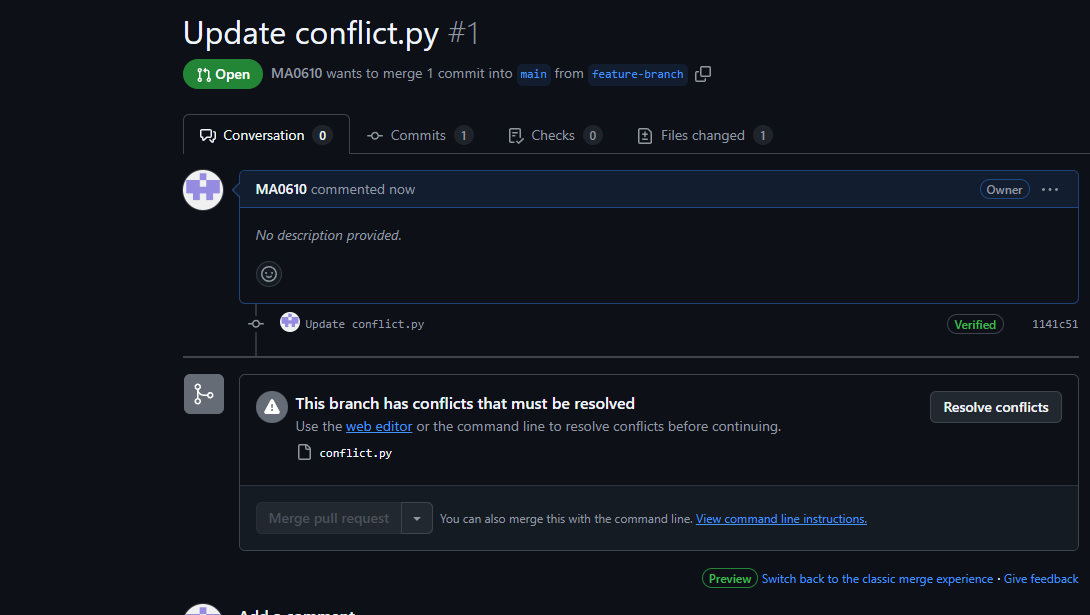
\includegraphics[width=\columnwidth]{Screenshot 2025-03-03 211752.png}
    \caption{In this file I changed the functionTest() function to where it returned different values/did different things}
    \label{fig:alrc}
    \footnotesize
    \vspace{\baselineskip}
\end{figure}

\end{enumerate}

\subsection{Remotes}

\begin{enumerate}
\item What is a remote?
\subitem A remote is a remote repository. It is a repository that is hosted on the Internet/a network.

\item What does pushing and pulling do?
\subitem Pushing uploads the commits that are local to the remote repository. Meanwhile pulling downloads the changes from the remote repository and merges them to the local branch.

\item Imagine you created a git repository for your project on your laptop and commit regularly, but only push your code to GitHub once a week on Sundays. Your laptop caught on fire on Friday. What can you do to get your code back?
\subitem The best I could do is get the code from the last push that I had made from the previous Sunday. I would be able to clone the repository doing git clone githubLinkHere.

\end{enumerate}

\section{\LaTeX}

Find a source of each of the following types and add it to \texttt{references.bib}, with the appropriate data. Your sources do not have to relate to your project. Looking at \textcite{OverleafBibliographyManagement} and \textcite{WikipediaBibtex} may be helpful,

\begin{itemize}
\item a journal article
\subitem \cite{hoadley_using_2005}

\item a conference article
\subitem \cite{huang_how_2023}

\item a PhD or Master's thesis
\subitem \cite{noauthor_phd_nodate}

\item an article in an edited popular media venue (newspaper, magazine, etc.)
\subitem \cite{noauthor_microsoft_nodate}

\item a book
\subitem \cite{shackelford_forks_2023}

\item a chapter of a book
\subitem \cite{sugiki_ocean_2022}

\item a YouTube video
\subitem \cite{noauthor_react_nodate}

\item a piece of technical documentation (e.g., a programming language reference, and API documentation, etc.)
\subitem \cite{noauthor_react_nodate-1}

\end{itemize}

Additionally, in you own words, explain the difference between \texttt{{\textbackslash}cite\{\}} and \texttt{{\textbackslash}textcite\{\}}. When should they each be used? Demonstrate your answers by using one of them with each of your references from above.

\subitem Textcite cites brings the citation within the sentence which allows for the sentence to incorporate the source including author names within the actual paper. Meanwhile cite places the citation towards the end and should be done when just wanting to deal with multiple citations or just making a general reference towards the source. This is an example of me using\textcite{hoadley_using_2005}. And here is me using the Huang article \cite{huang_how_2023}.



\printbibliography

\end{document}
